%%================================================
%% Filename: chap03.tex
%% Encoding: UTF-8
%% Author: Yuan Xiaoshuai - yxshuai@gmail.com
%% Created: 2012-04-27 19:47
%% Last modified: 2016-09-02 21:31
%%================================================
\chapter{第三章 系统设计}
\label{cha:usage}

\section{系统布局}
\label{sec:requirements}

考虑到本系统的复杂性,与基于每个社团的需求不一,所以将每个系统单独出来,各个完成。如有些社团仅需要报名与值班系统,我只要为你部署这两个系统即可,数据通过 CSV 表格形式进行人为传输。确保数据的可靠性与流动性。其次考虑到每个系统环境不一样,所以利用简单的 Docker 配置,可以一次性的安装多个系统。方便一些操作人员操作。

由于每个系统功能都有很大差别,所以系统设计每个模块都有不同的技术选型,一来,每个技术都有自己适合的领域,使开发方便又不容易出错。二来,尝试不同的技术,可以很好的察觉不同技术之间的差距,避免以后犯一些技术选型错误。三来,每个技术都可以展现自己不同时期学习的情况,也同样反应新技术更迭速度快,需要我们更快的理解新技术的诞生与发展趋势。

以下我会以技术选型的不同,分别介绍这六大系统模块。这三大技术,分别是:
\begin{itemize}
  \item 以 PHP 和 MySQL 为基础的 ThinkPHP3.2 版本框架(报名系统与考核系统)
  \item 以 JavaScript 为基础的 Express 和 Pug 框架(群发短信平台,学习平台,值班系统)
  \item 以 JavaScript 为基础的,以前后端分离为思想的 Vue 前端框架与 Koa 后端接口框架(邮件群发平台)
\end{itemize}

\section{技术选型}
\label{sec:requirements}

\subsection{ThinkPHP3.2 框架}
\label{sec:requirements}

ThinkPHP 是以 PHP 为底层的框架。相较于其他 Laravel,Yii,Zend 等大型框架,ThinkPHP 框架属于轻量型框架,没有什么特殊模块要求,底层运行的内容消耗也很低,不会出现空间和内存占用的瓶颈。并且它支持 Mysql、MsSQL、PgSQL、Sqlite、Oracle、Ibase、Mongo以及PDO等多种数据库和连接。对于这种一般型的项目足以。

\subsubsection*{项目后端的搭建}

\begin{itemize}
  \item 使用 PHP 语言的 ThinkPHP3.2 框架完成网站后端搭建
  \item 使用 mysql 完成数据存储,通过 model 模块完成对 mysql 数据的构建使用 thinkphp 模板引擎完成页面创建渲染
  \item 使用 ThinkPHP的 关联模型构建关系型模型
\end{itemize}

\subsubsection*{项目前端搭建}

\begin{itemize}
  \item 使用 jQuery 和 Bootsrap 完成网站前端JS脚本和样式处理
  \item 使用 jQuery.min.js 完成对账号以及选项的判断
  \item 前后端的数据请求交互通过Ajax完成
\end{itemize}

\subsubsection{报名管理系统}
\label{sec:requirements}

\subsubsection*{设计}

项目相关设计 UI 如图~\ref{fig:04-01-signinsys}~,~\ref{fig:04-02-signinsys}~,~\ref{fig:04-03-signinsys}~所示

\begin{figure}[htbp]
\centering
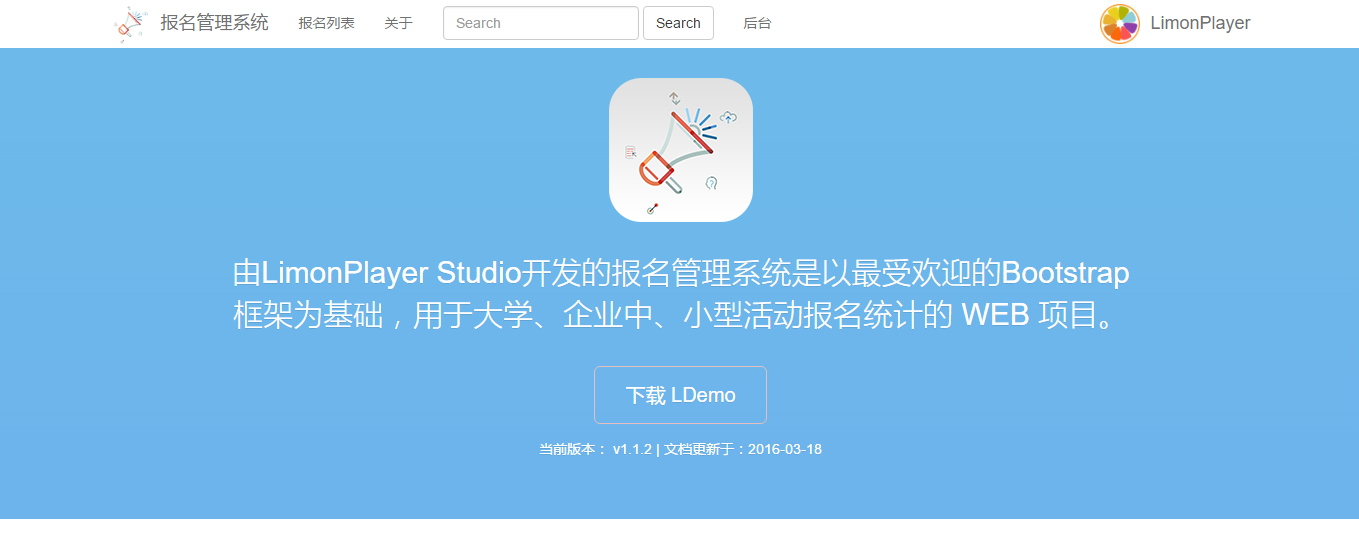
\includegraphics[width=0.7\textwidth]{04-01-signinsys}
\caption{报名首页}
\label{fig:04-01-signinsys}
\end{figure}

\begin{figure}[htbp]
\centering
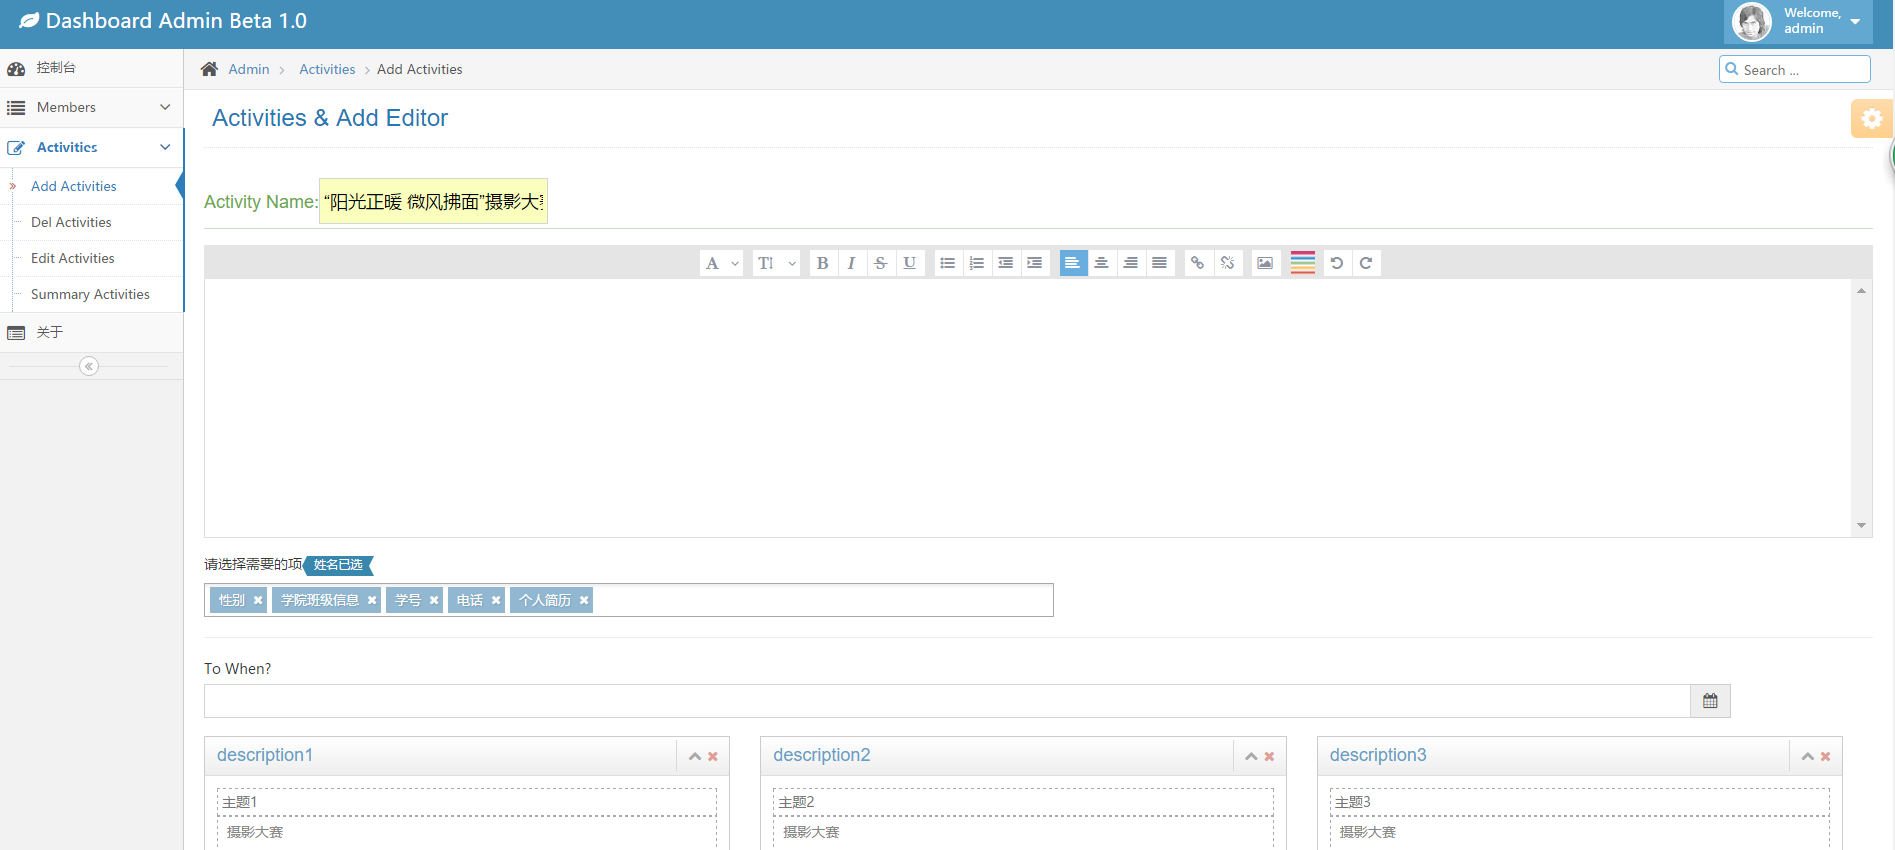
\includegraphics[width=0.7\textwidth]{04-02-signinsys}
\caption{后台管理页}
\label{fig:04-02-signinsys}
\end{figure}

\begin{figure}[htbp]
\centering
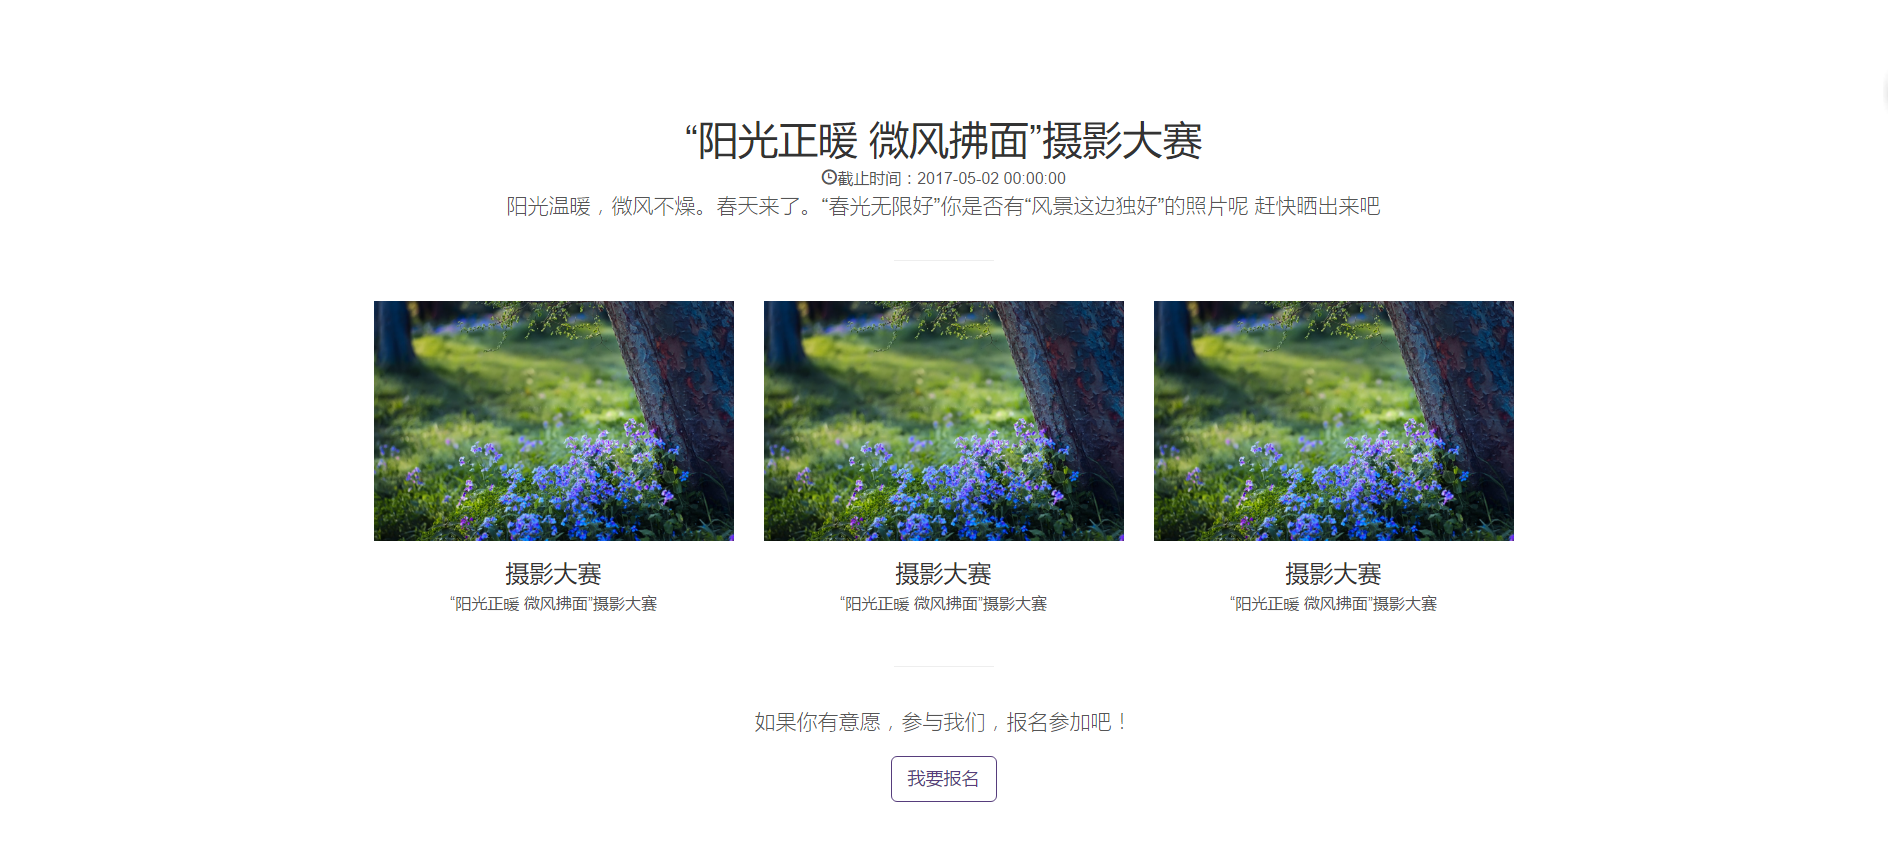
\includegraphics[width=0.7\textwidth]{04-03-signinsys}
\caption{报名列表页}
\label{fig:04-03-signinsys}
\end{figure}

\subsubsection*{详细功能}

本项目主要有活动活动的创建与 excel 导出功能,其次有对活动时间的控制,可以对活动进行修改,富文本的编辑与操作。

\subsubsection{考核系统}
\label{sec:requirements}

\subsubsection*{设计}

项目相关设计 UI 如图~\ref{fig:04-04-exam-sys}~,~\ref{fig:04-05-exam-sys}~所示

\begin{figure}[htbp]
\centering
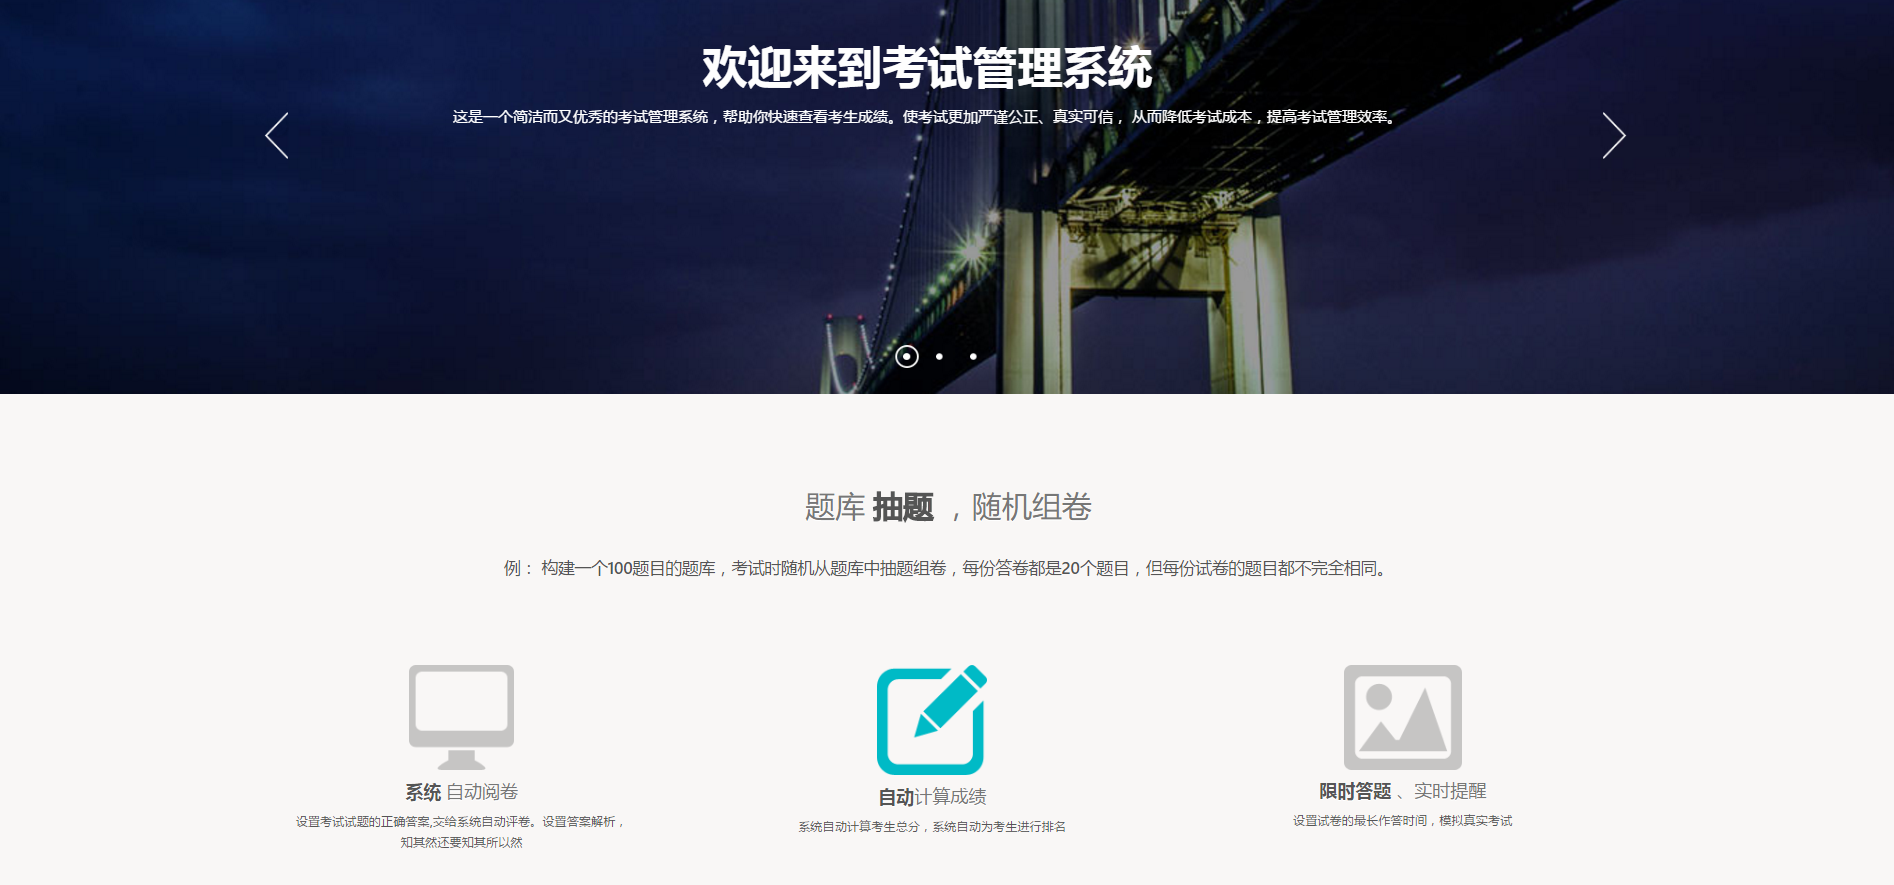
\includegraphics[width=0.7\textwidth]{04-04-exam-sys}
\caption{项目首页}
\label{fig:04-04-exam-sys}
\end{figure}

\begin{figure}[htbp]
\centering
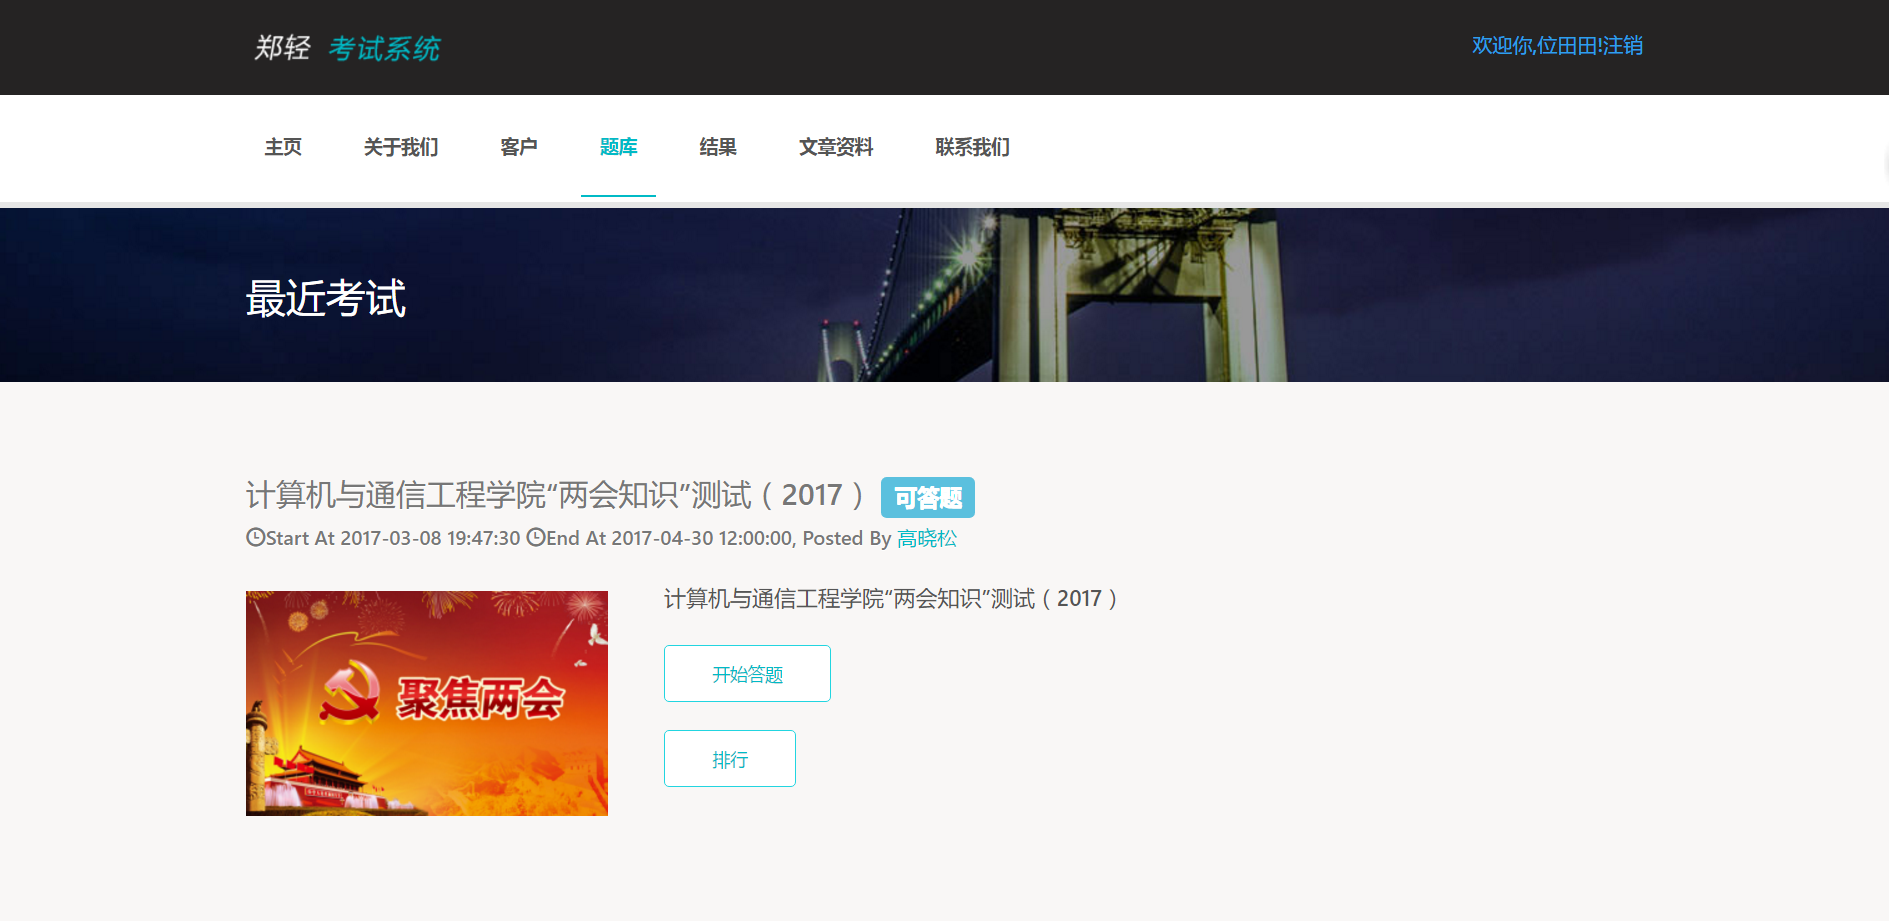
\includegraphics[width=0.7\textwidth]{04-05-exam-sys}
\caption{选择考试页}
\label{fig:04-05-exam-sys}
\end{figure}

\subsubsection*{详细功能}

本项目主要由试卷 exam 和文章 article 两大模型
\begin{itemize}
  \item 其中具有重要特色的功能是对试卷的添加与编辑和批改等功能
  \item 其次在克服试卷的模型上我们做了很多尝试,最后用了稳定而不易出错的 thinkphp 自带关联模型
  \item 对用户的考试成绩进行排序rank(可以比较出学员的优异性)
  \item 对考试时间的设定与修改
  \item 还有对大量用户数据的批量处理
  \item 对用户的权限处理
\end{itemize}

\subsection{Express 与 Pug 框架}

\subsubsection*{项目后端的搭建}
\begin{itemize}
  \item 使用 NodeJs 的 express 框架完成网站后端搭建
  \item 使用 mongodb 完成数据存储,通过 mongoose 模块完成对 mongodb 数据的构建使用 pug 模板引擎完成页面创建渲染
  \item 使用 Moment.js 格式化电影存储时间
  \item 利用 alibaba.aliqin.fc.sms.num.send(短信发送)收费API作为发短信支持
\end{itemize}

\subsubsection*{项目前端搭建}

\begin{itemize}
  \item 使用 jQuery 和 Bootsrap 完成网站前端JS脚本和样式处理
  \item 使用 jQuery.min.js 完成对账号以及选项的判断
  \item 前后端的数据请求交互通过 Ajax 完成
  \item 前端的页面渲染通过 PUG 最新插件完成
  \item 跨域的数据请求交互通过 Ajax 中的 jsonp 完成
\end{itemize}

\subsubsection{短信群发平台}
\label{sec:requirements}

\subsubsection*{设计}

项目相关设计 UI 如图~\ref{fig:04-06-sms}~,~\ref{fig:04-07-sms}~,~\ref{fig:04-08-sms}~所示

\begin{figure}[htbp]
\centering
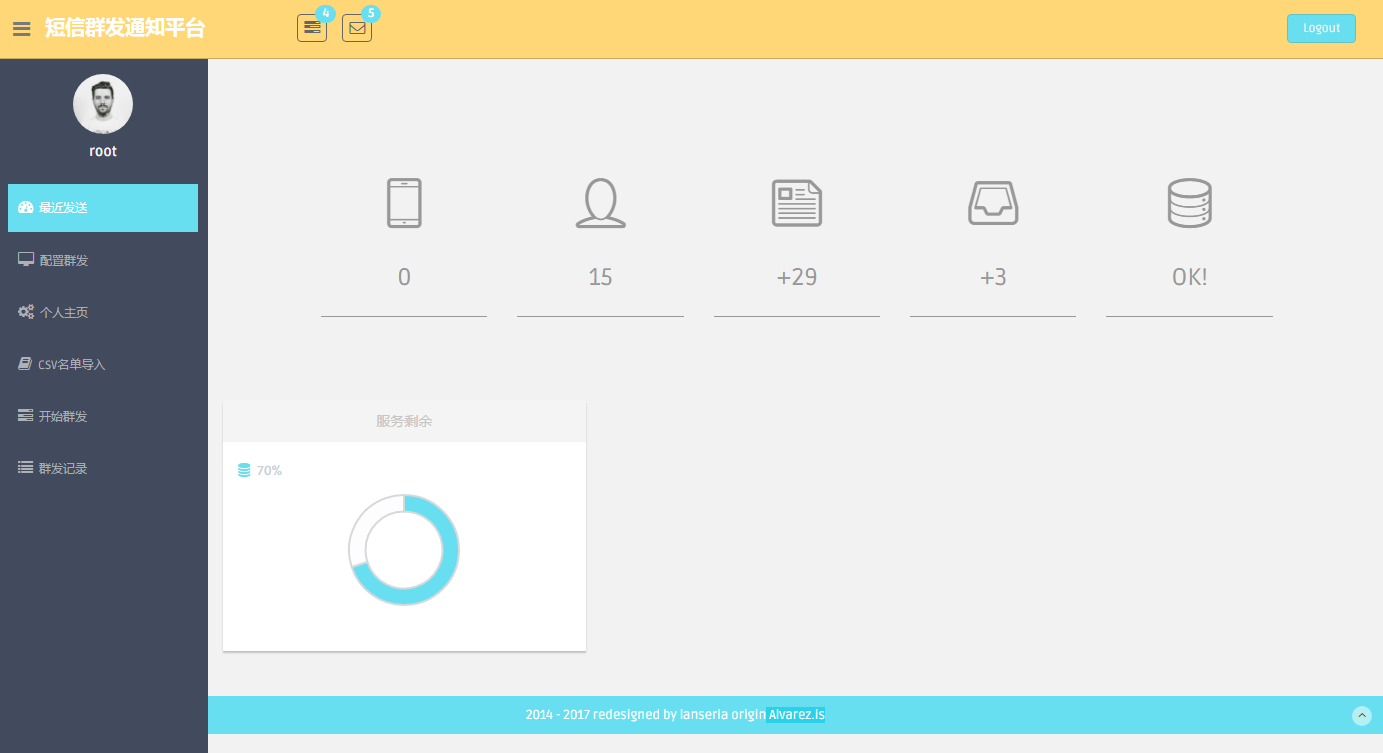
\includegraphics[width=0.7\textwidth]{04-06-sms}
\caption{项目首页}
\label{fig:04-06-sms}
\end{figure}

\begin{figure}[htbp]
\centering
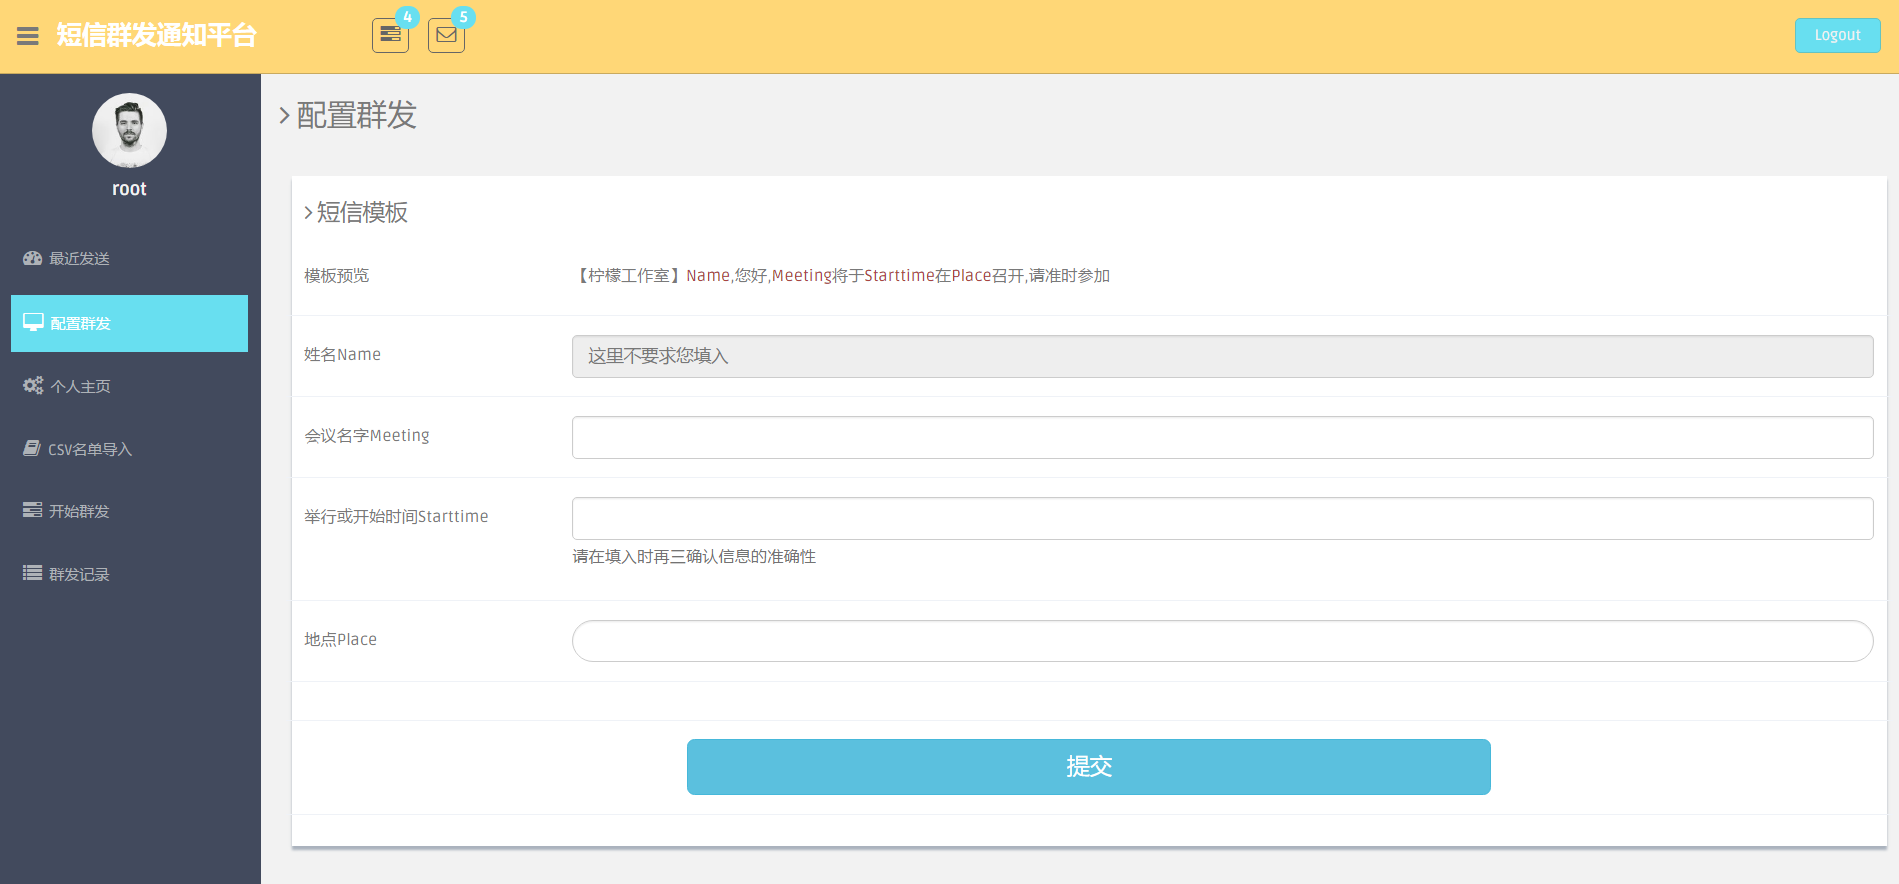
\includegraphics[width=0.7\textwidth]{04-07-sms}
\caption{模板信息填写页}
\label{fig:04-07-sms}
\end{figure}

\begin{figure}[htbp]
\centering
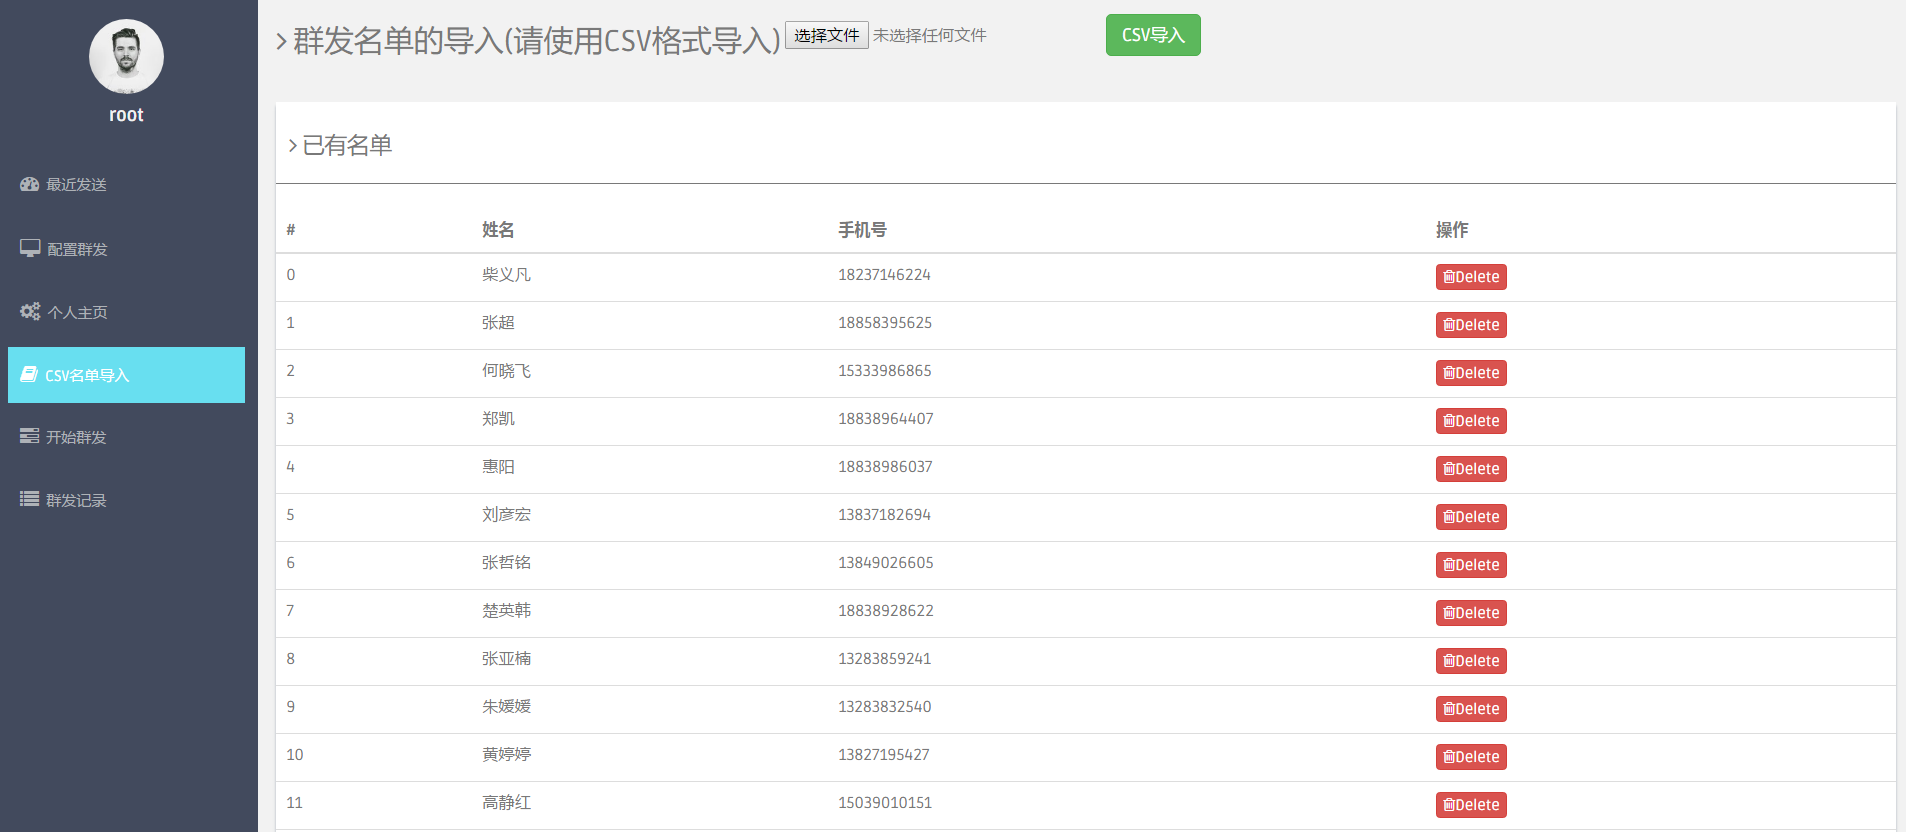
\includegraphics[width=0.7\textwidth]{04-08-sms}
\caption{信息群发页}
\label{fig:04-08-sms}
\end{figure}

\subsubsection*{详细功能}

本项目主要由 CSV 名单导入和短信群 smsMass 发两大功能
\begin{itemize}
  \item 其中具有重要特色的功能是对权限的控制上附加了对申请 key 的操作
  \item 其次在短信模板上可以自己相应的信息,进行合理的增删改查与默认的功能
  \item 对短信群发的信息有日志的记录log
  \item 对用户的权限处理
\end{itemize}

\subsubsection{排值班系统}
\label{sec:requirements}

\subsubsection*{设计}

项目相关设计 UI 如图~\ref{fig:04-09-arr}~所示

\begin{figure}[htbp]
\centering
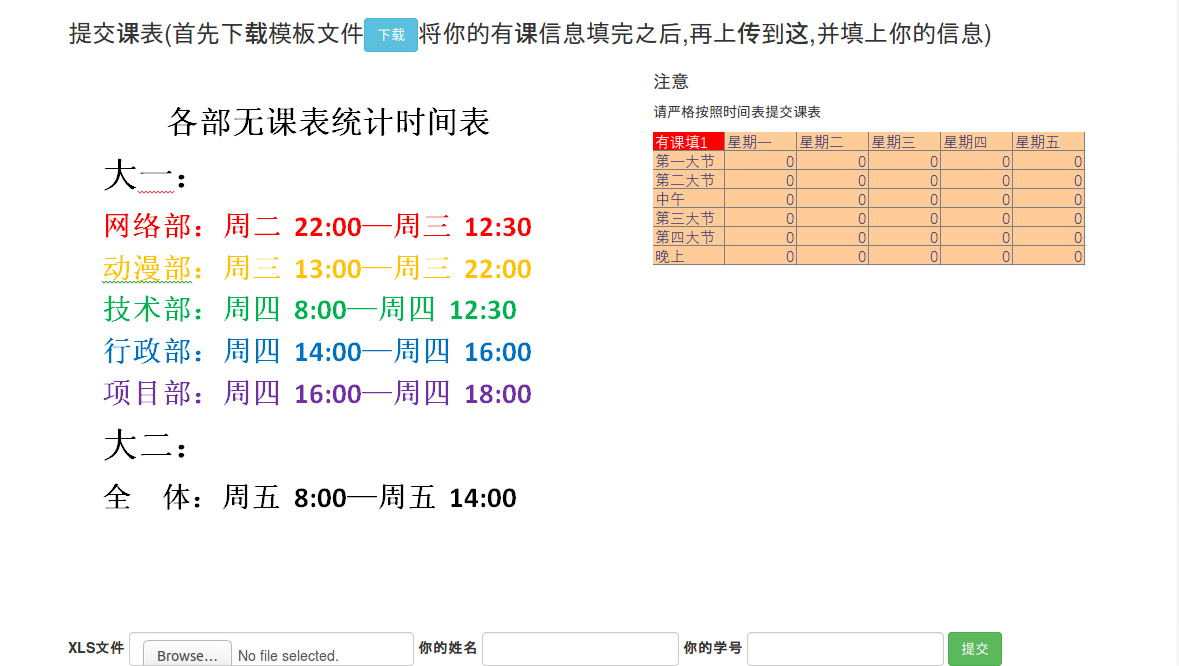
\includegraphics[width=0.7\textwidth]{04-09-arr}
\caption{首页}
\label{fig:04-09-arr}
\end{figure}

\subsubsection*{详细功能}

排值班系统是一套集成C/C++暴力算法排序的,集成 xlsx 的导入与导出制作的一套系统。通过人编写的算法,对成员的值班表进行进行智能的分析,以不重复安排一个人的前提下,尽量将每个成员分配上去,以保证公平,公正。但是最主要的是减少人工排课的工作量,方便管理员的导入导出与使用。

\subsubsection{学习平台}
\label{sec:requirements}

\subsubsection*{设计}

项目相关设计 UI 如图~\ref{fig:04-10-learn}~,~\ref{fig:04-11-learn}~所示

\begin{figure}[htbp]
\centering
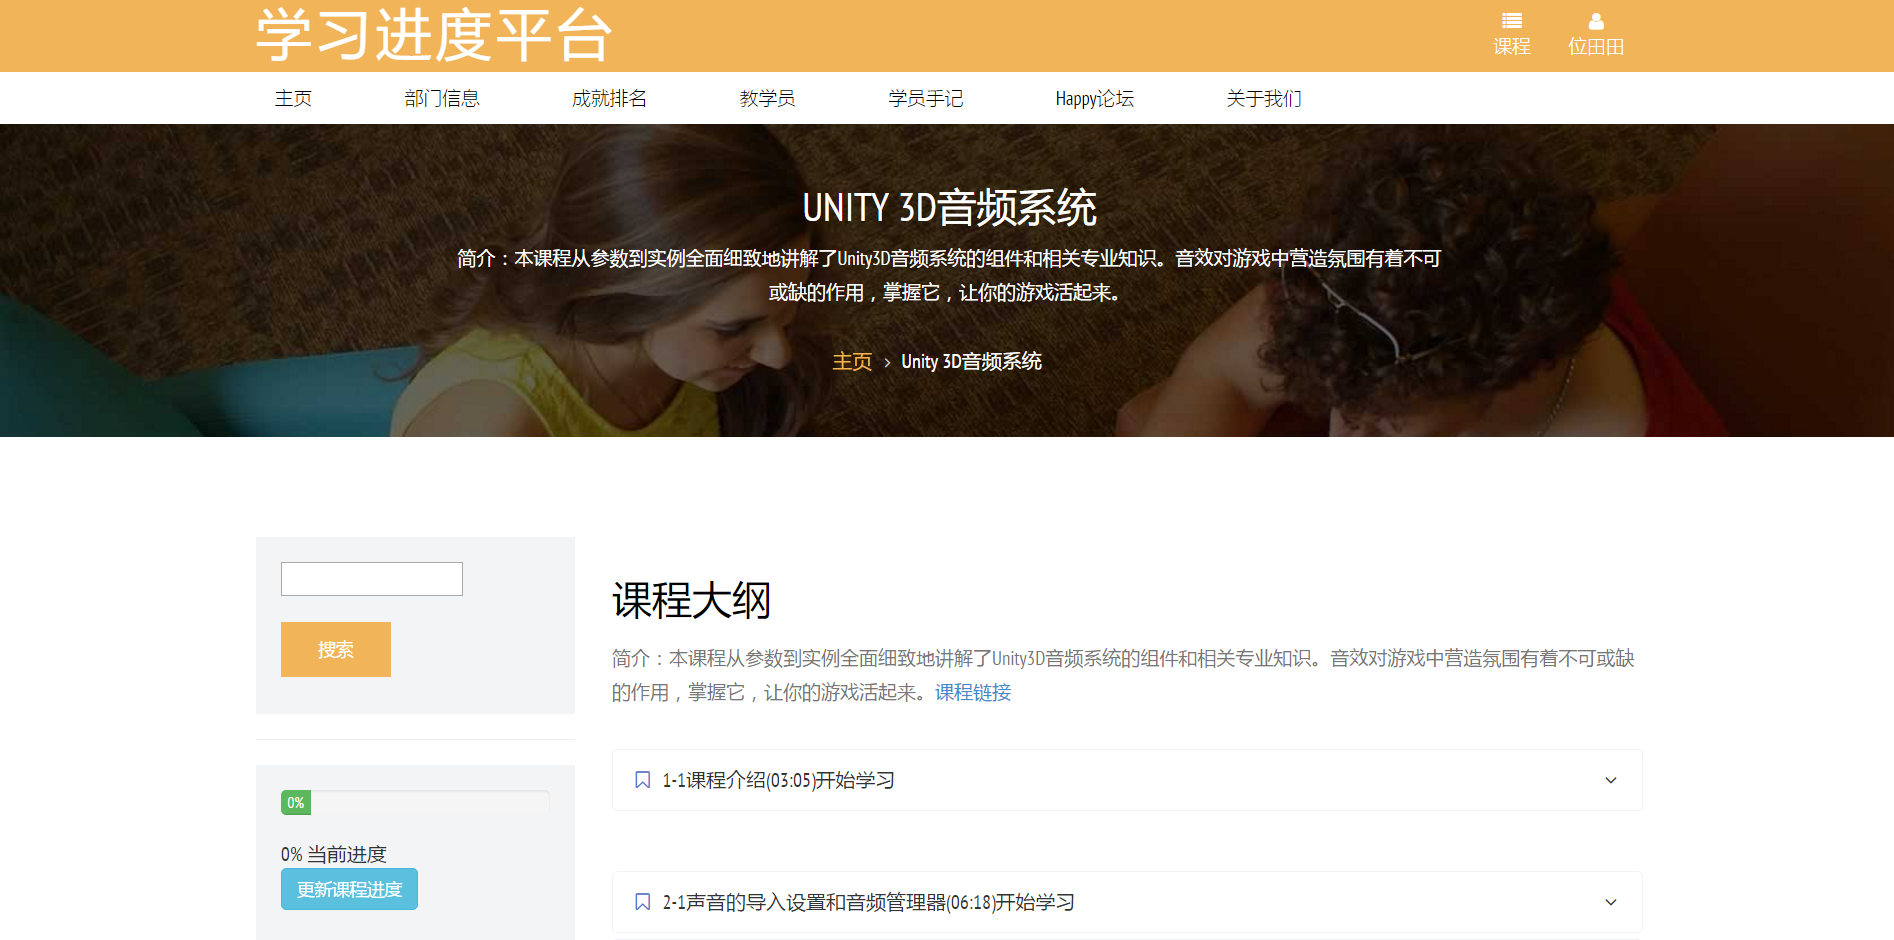
\includegraphics[width=0.7\textwidth]{04-10-learn}
\caption{课程页}
\label{fig:04-10-learn}
\end{figure}

\begin{figure}[htbp]
\centering
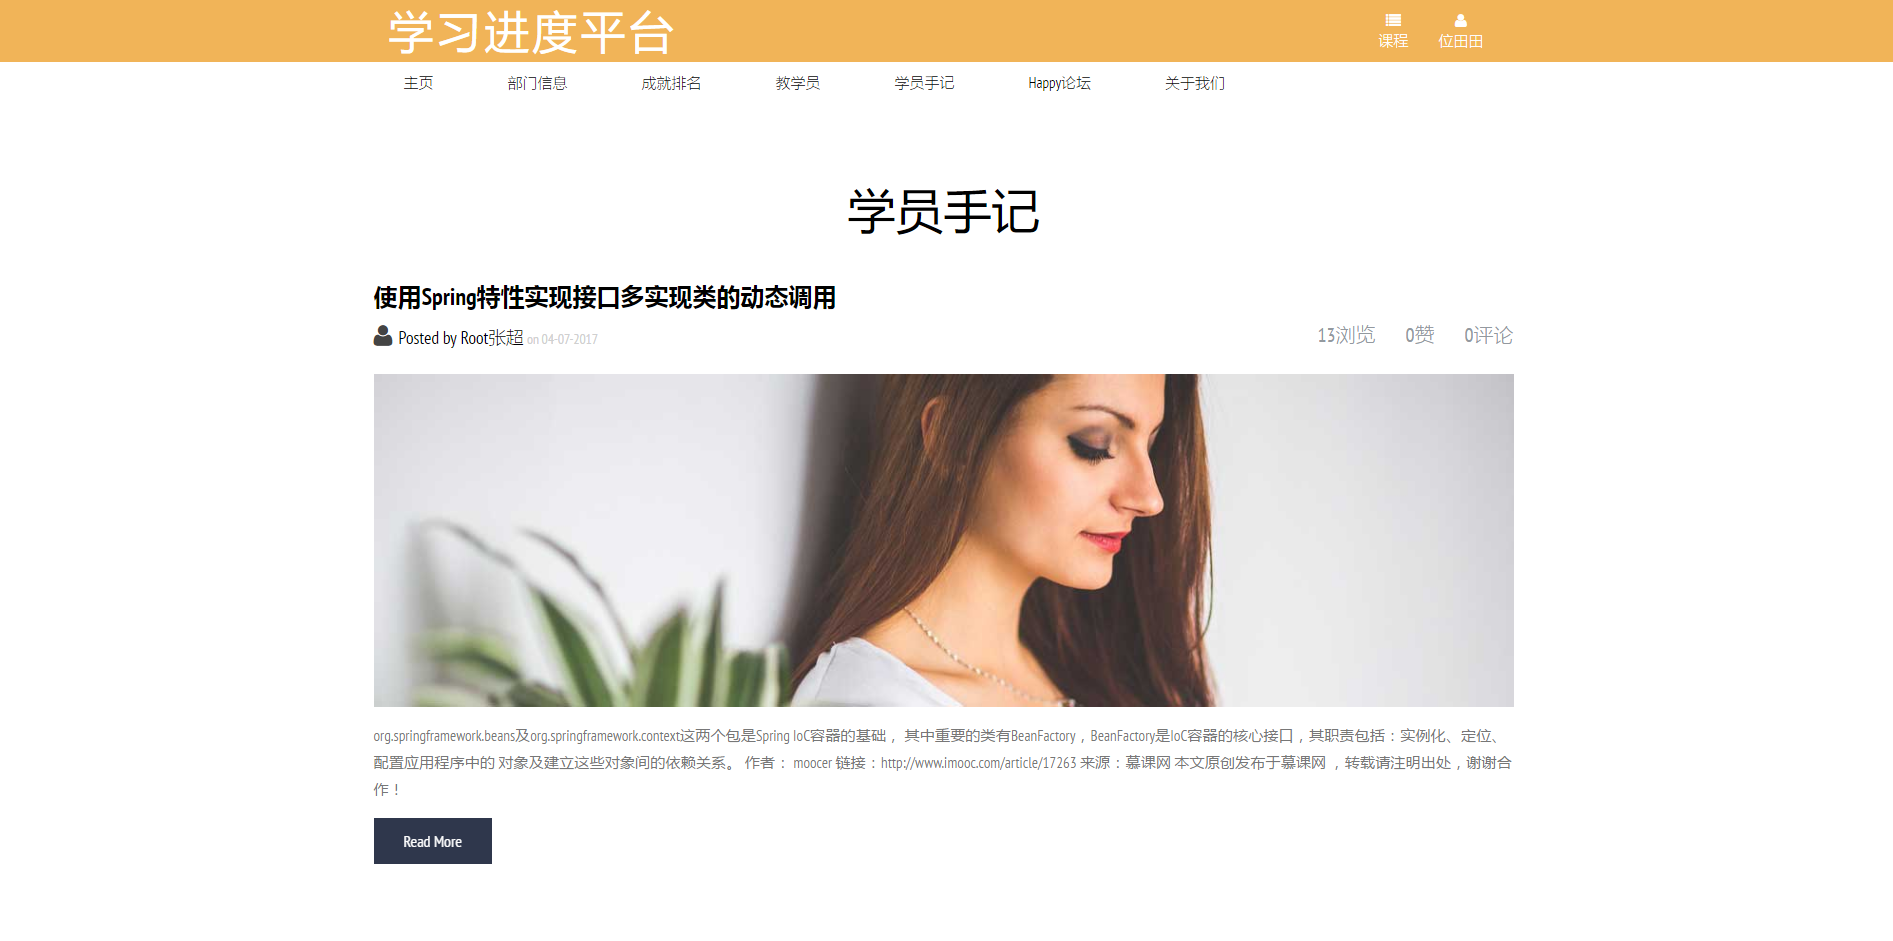
\includegraphics[width=0.7\textwidth]{04-11-learn}
\caption{手记页}
\label{fig:04-11-learn}
\end{figure}

\subsubsection*{详细功能}

本项目由学习进度 course 和文章发表 article 两大功能。
\begin{itemize}
  \item 其中具有重要特色的功能是慕课网信息的爬取与使用 spider,利用superagent插件。
  \item 其次具有简单的用户登录和注册 user ,用户的头像上传
  \item 对用户的学习进度进行排序 rank (可以比较出学员的积极性)
  \item 对课程 course 的搜索 search
  \item 还有对每个列表页面进行分页 page 处理
  \item 访客次数统计 pv
\end{itemize}

\subsection{Vue 与 Koa 前后端分离}
\label{sec:requirements}

\subsubsection{邮件发送平台}
\label{sec:requirements}

\subsubsection*{设计}

项目相关设计 UI 如图~\ref{fig:04-12-email}~所示

\begin{figure}[htbp]
\centering
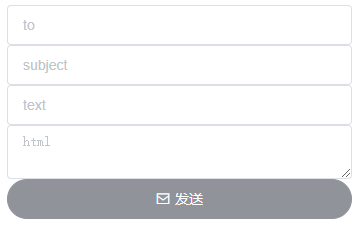
\includegraphics[width=0.7\textwidth]{04-12-email}
\caption{发送页}
\label{fig:04-12-email}
\end{figure}

\subsubsection*{详细功能}

本项目利用 nodemailer 和 QQ 邮箱的 STMP 利用,加上独特的域名配置,可以实现简单的 HTML 格式邮件发送。

